\section{Synthesis}
\begin{figure}
    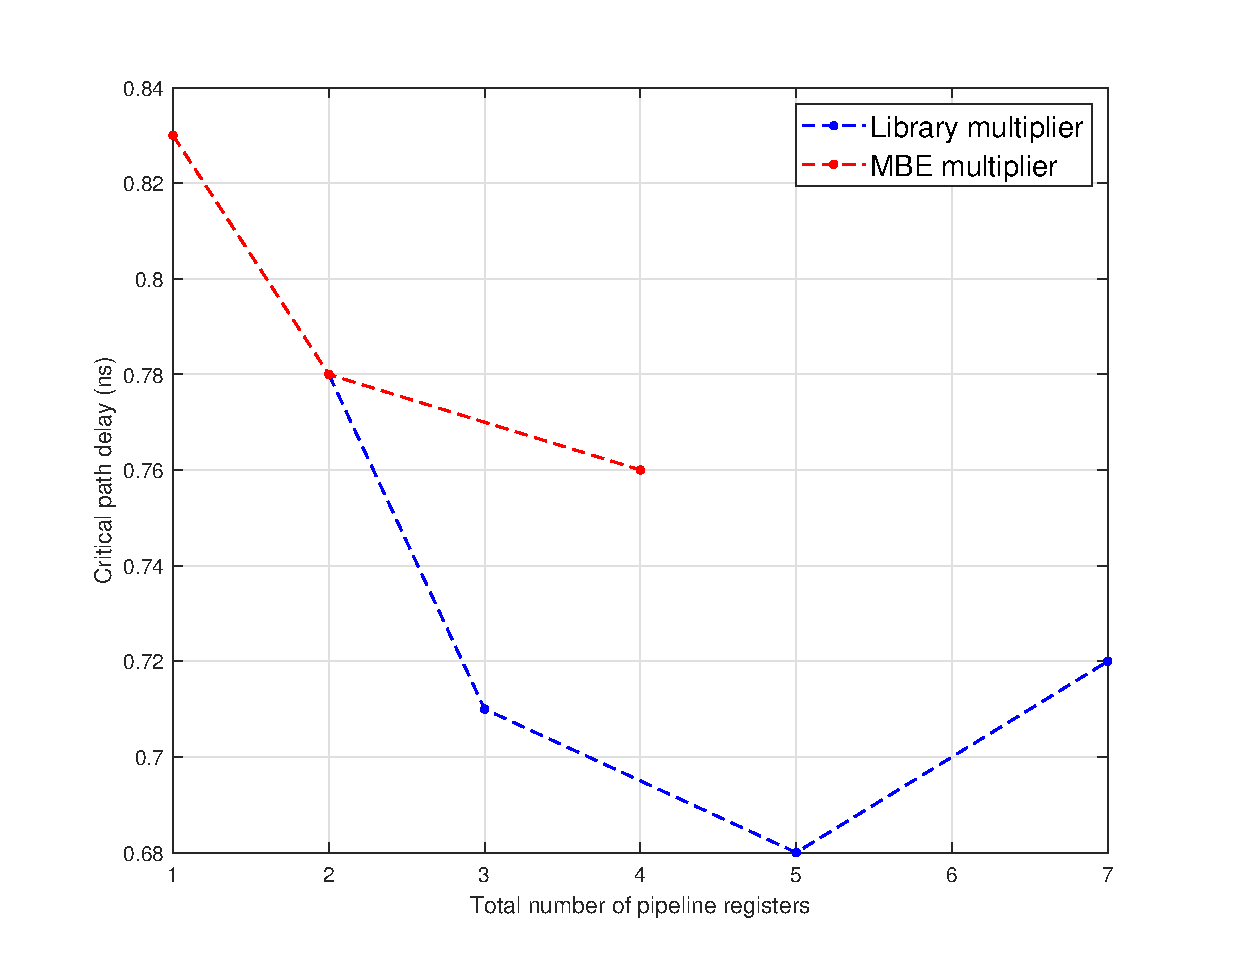
\includegraphics[width=\textwidth]{chapter2/images/delays.eps}
    \caption{Critical path delays as a function of total number of pipeline registers}
    \label{fig:delays}
\end{figure}
This new multiplier replaces the library multiplier instantiated in the second stage of \texttt{fpmul}. In order to fairly assess the impact that this component has on performance, pipeline registers are included and the synthesis process is repeated with several values of \texttt{NPIPE}, the constant denoting the number of pipeline registers.
\begin{table}[htbp]
\resizebox{\linewidth}{!}{
\begin{tabular}{|l|l|l|l|l|l|l|}\hline
    & No retiming & \texttt{NPIPE=1} & \texttt{NPIPE=2} & \texttt{NPIPE=4} & \texttt{NPIPE=6} & \texttt{NPIPE=8}\\\hline
    Clock period & $\SI{1.44}{ns}$ & $\SI{0.83}{ns}$ & $\SI{0.78}{ns}$ & $\SI{0.76}{ns}$ & $\SI{0.71}{ns}$& 0.68$\,\textrm{ns}$ \\\hline
    Total area  (\SI{}{\micro m^2}) & 5935 & 6926 & 7130 & 7992 & 8402 & 8273 \\\hline
    Combinational area  (\SI{}{\micro m^2}) & 4794 & 4842 & 4655 & 4749 & 4729 & 4657 \\\hline
    Area (\texttt{mbe\_mult/add\_1424}) & 372 (6.3 \%)  & 419 (6 \%)  &  705 (9.9 \%)& 654 (8.2 \%) & 648 (7.7 \%) & 643 (7.8 \%)\\\hline
\end{tabular}
}
\caption{Characterization of the MBE multiplier}
\label{tab:MBE}
\end{table}

\autoref{fig:delays} shows that the MBE multiplier can potentially reach the same critical path delay as the library one, provided that more pipeline stages are inserted. This plot shows that there is an optimum number of pipeline stages, beyond which it is no longer possible to break critical paths using this technique. The MBE design reaches the minimum critical path delay with eight registers, whereas four stages are the best choice when resorting to the DesignWare component. Designs that include the MBE multiplier have been synthesized using a larger total area, as apparent by comparing \autoref{tab:MBE} with \autoref{tab:stage2}.

\begin{table}
    \centering
    \begin{tabular}{|lrr|}\hline
        Point                        & Incr  & Path  \\
        \hline
        clock clk (rise edge)        &  0.00 &  0.00 \\
        clock network delay (ideal)  &  0.00 &  0.00 \\
        clk\_r\_REG18\_S9/CK         &  0.00 &  0.00 \\
        clk\_r\_REG18\_S9/Q          &  0.09 &  0.09 \\
        FP\_Z[0] (out)               &  0.02 &  0.11 \\
        data arrival time            &       &  0.11 \\
        \hline
        clock clk (rise edge)        &  0.00 &  0.00 \\
        clock network delay (ideal)  &  0.00 &  0.00 \\
        clock uncertainty            & -0.07 & -0.07 \\
        output external delay        & -0.50 & -0.57 \\
        \hline
        data required time           &       & -0.57 \\
        data required time           &       & -0.57 \\
        data arrival time            &       & -0.11 \\
        \hline
        slack (VIOLATED)             &       & -0.68 \\
        \hline
    \end{tabular}
    \caption{Timing report obtained with a value of exttt{NPIPE} that minimizes overall delay looks the same in both cases (MBE and Designware)}
    \label{tab:report}
\end{table}

It is interesting to note that timing reports (\autoref{tab:report}) obtained in the condition where minimum delay is achieved are the same for the two designs compared in \autoref{fig:delays}. They both consist in a clock-to-output delay that amounts to 0.11 ns, only a fraction of the fixed delay due to clock uncertainty (set to 0.07) and input/output delays (set to 0.5) set in the synthesis script to model a real situation. This shows that in both cases the retiming tool is able to reach the very minimum delay allowed by the available library and the specified uncertainties.
